% Took this from CogSci but removed the header, sorry.
%
% Author: Matthew Turner
% Date: 2017-11-23

\documentclass[11pt,letterpaper]{article}

% \usepackage{cogsci}
\usepackage{fullpage}
\usepackage{booktabs}
\usepackage{pslatex}
\usepackage{apacite}
\usepackage{amsmath}
\usepackage{subcaption}
\usepackage[utf8]{inputenc}
\usepackage{pgfplots}
\pgfplotsset{compat=newest}
\usepgfplotslibrary{groupplots}
\usepackage{wrapfig}
% \usepackage{url}
% \usepackage{hyperref}
\usepackage{bigfoot}
\usepackage[export]{adjustbox}
\setlength\intextsep{0pt}



\usepackage{graphicx}

\usepackage{gb4e}  % linguistic examples
\noautomath

\title{Reproduction of Flache and Macy 2011 experiment two with negative valence}

\author{{\bf Matthew A.~Turner (mturner8@ucmerced.edu)}}

\begin{document}
\maketitle

\begin{abstract}
  Opinion dynamics in general models how attributes of agents in a population
  change over time. This paper reproduces and extends the investigation of
  \citeA{Flache2011} into how cultural polarization emerges in populations
  connected on a small-world network. Their results do much to shed light
  on what might be the necessary requirements for polarization to occur.
  Importantly, opinions must be measured in a way that allows for negative
  valence of opinion, representing being ``against'' some cultural object.
  Here we add three further considerations we believe are important in 
  modeling when polarization obtains. First, we show that final polarization
  is sensitive to the initial extremity of agent opinions. Second, we quantify
  how robust polarizing dynamics are to noise. Finally, we try to more deeply
  understand the effect of increasing the dimensionality of agent opinion
  vectors. \citeA{Flache2011} find that increasing $K$ results in the
  disappearance of polarizing dynamics. To address this, we argue that 
  Flache and Macy's distance metric may have unintended consequences that are
  exacerbated as $K$ increases and makes polarization unlikely given 
  uniformly distributed initial conditions for each element of the agent
  opinion vectors. We re-run Flache and Macy's experiments with
  alternative opinion distance measures, and discuss the pros and cons of their
  approach and the alternative measures we propose. Finally, we suggest that
  determining clusters and distance between clusters may be a more informative
  measure of the population's final state than polarization measure of 
  variance of distances as used by Flache and Macy.
\end{abstract}

\section{Outline}

\begin{enumerate}
  \item Experiment with changes in $S$ for $K=2, 3, 5$
  \item Argue for cosine distance and re-run all experiments with cosine distance for $d_{ij}$
  \item Add noise and re-run all experiments
  \item At this point, we have done many experiments, but we don't have a good
    feel for the dynamics that lead to the outcome measure. Also the outcome
    measure does not tell us much about the structure of agents. We could imagine
    situations where agents have clustered into more than two camps. 
    Let's explore the final configurations of a selection of experiments for
    higher dimensions.
\end{enumerate}

\section{Summary of Flache and Macy (2011) model}

\subsection{Expanded Figure 12b with additional $K$}
\begin{figure}
  \centering
      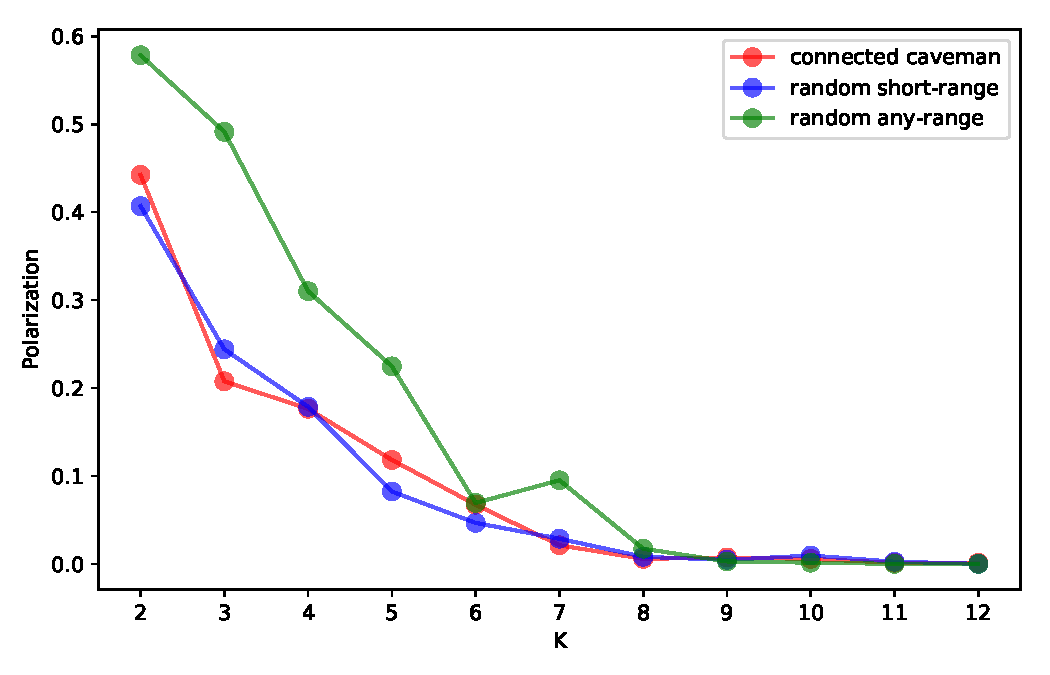
\includegraphics[width=0.75\textwidth]{Figures/finegrained_p_vs_K.pdf}
  \caption{
    Compare to FM 2011 Figure 12b. Identical, but with more intermediate
    values of cultural complexity $K$. As found by Flache and Macy, 
    average final polarization decreases with $K$. Each
    data point is the average of fifty trials. Each trial ran over 
    10k timesteps.
  }
  \label{fig:}
\end{figure}


\section{Effect of initial conditions on final polariztion}

\begin{figure}
  \centering
  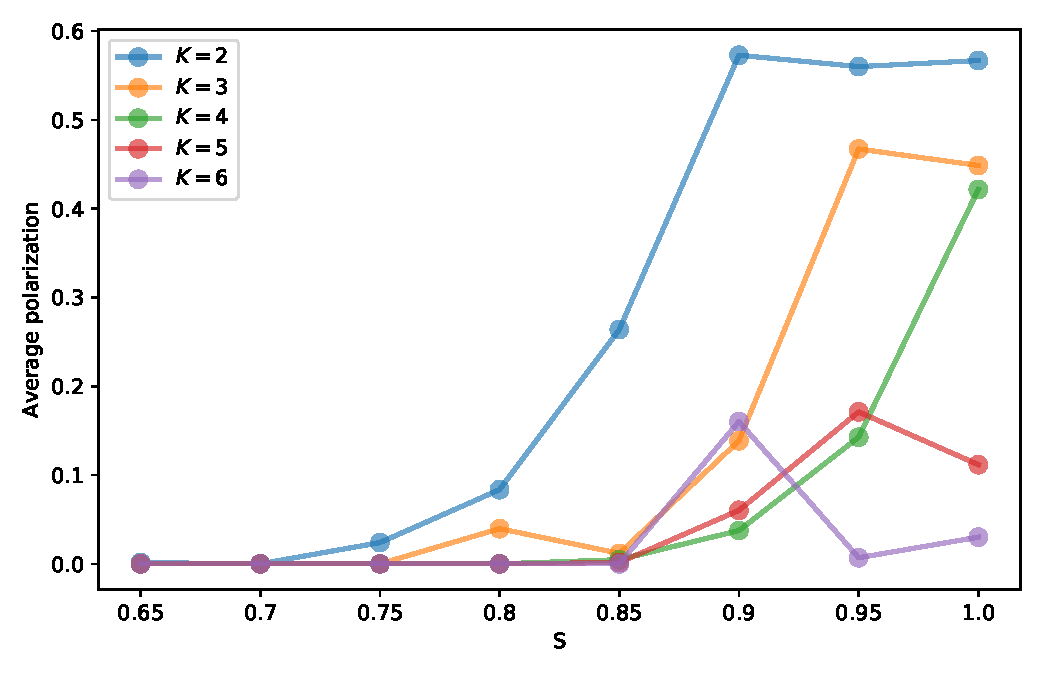
\includegraphics[width=0.75\textwidth]{Figures/P_vs_S_for_K.pdf}
  \caption{
    Average final polarization becomes non-zero then increases as
    the width of the uniform distribution of initial opinions increases.
    The width must be larger and larger as the cultural complexity $K$ 
    increases for the system to achieve non-zero final polarization. This
    condition is identical to the bottom row of each heatmap in 
    Figure \ref{fig:heatmaps}. Each
    data point is the average of fifty trials. Each trial ran over 
    10k timesteps. 
  }
  \label{fig:p_vs_s_for_k}
\end{figure}

\section{Effect of opinion update noise on final polarization}

\begin{figure}[t!]
  \centering
      \begin{subfigure}[t]{0.49\textwidth}
          \centering
          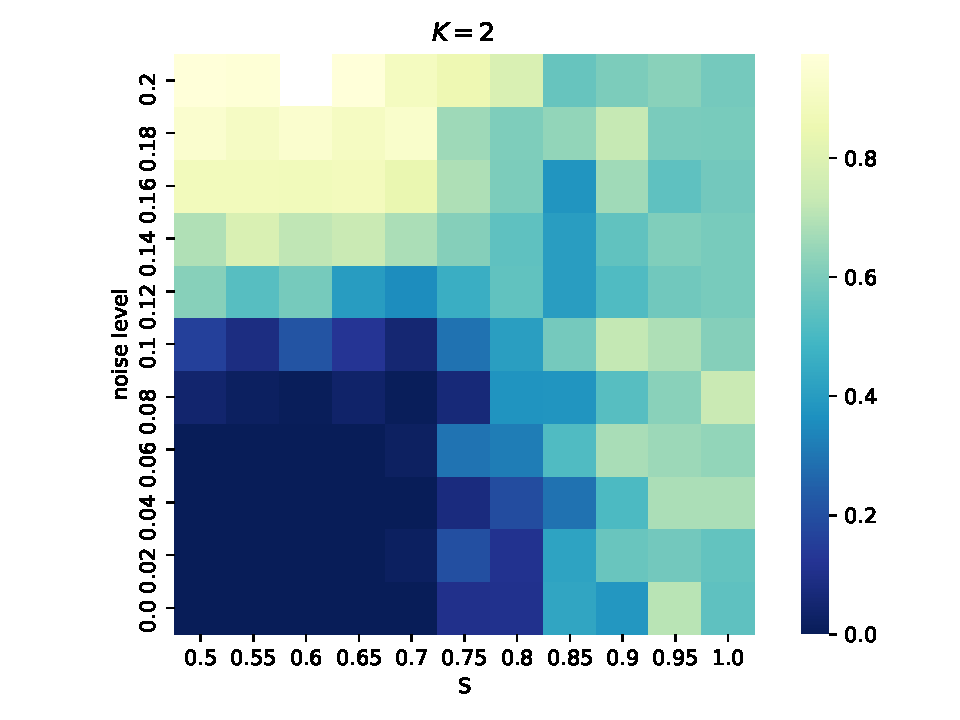
\includegraphics[width=\textwidth]{Figures/p_v_noise_k=2.pdf}
          \caption{}
      \end{subfigure}
      ~
      \begin{subfigure}[t]{0.49\textwidth}
          \centering
          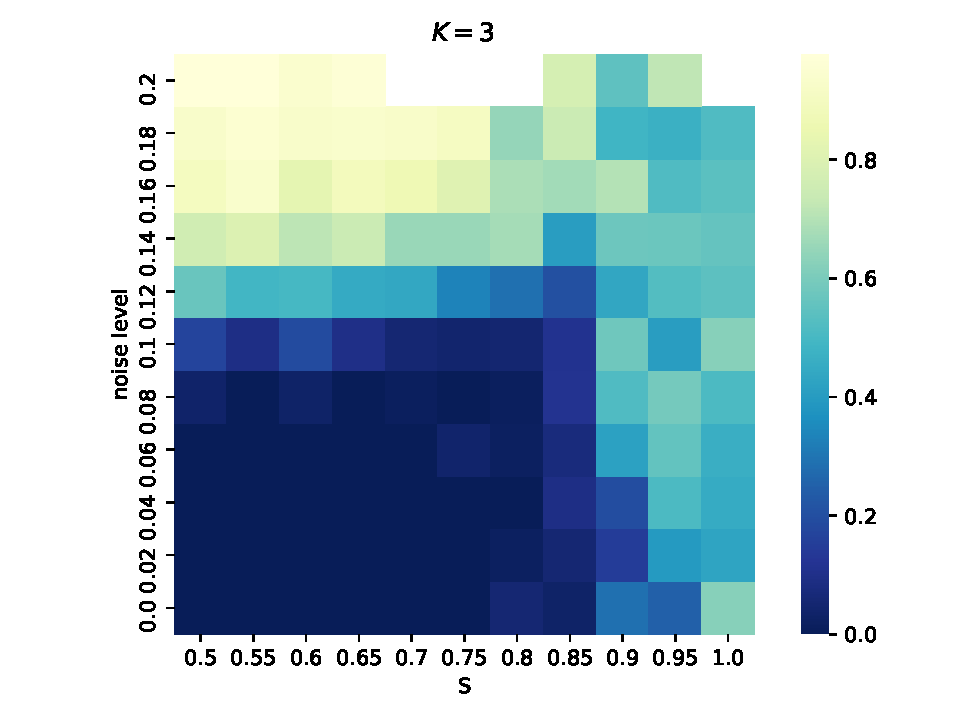
\includegraphics[width=\textwidth]{Figures/p_v_noise_k=3.pdf}
          \caption{}
      \end{subfigure} \\
      \begin{subfigure}[t]{0.49\textwidth}
          \centering
          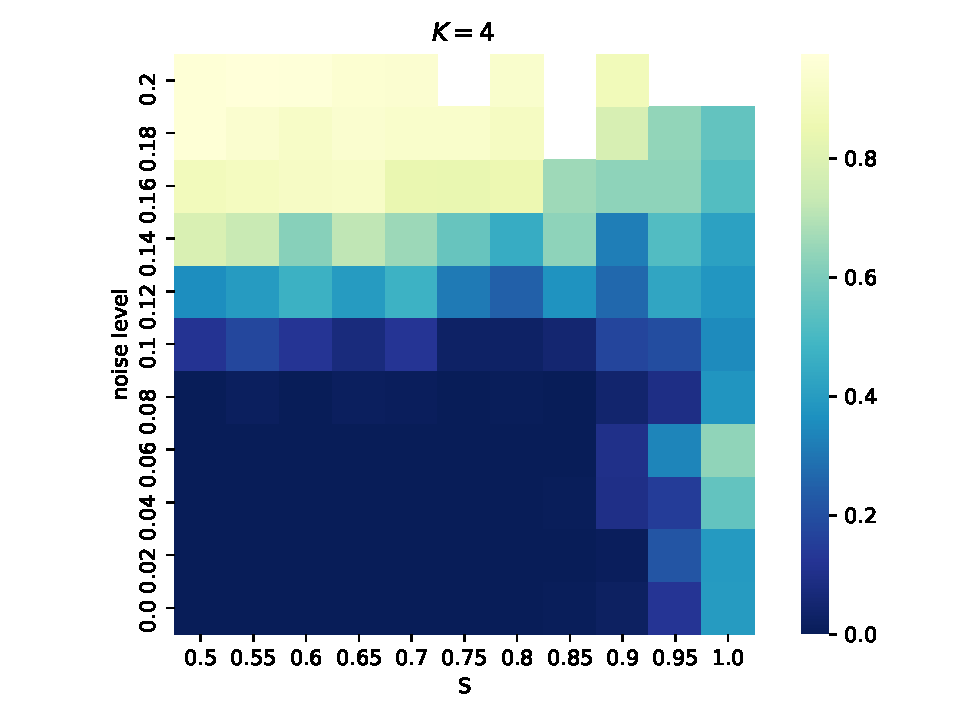
\includegraphics[width=\textwidth]{Figures/p_v_noise_k=4.pdf}
          \caption{}
      \end{subfigure}
      ~
      \begin{subfigure}[t]{0.49\textwidth}
          \centering
          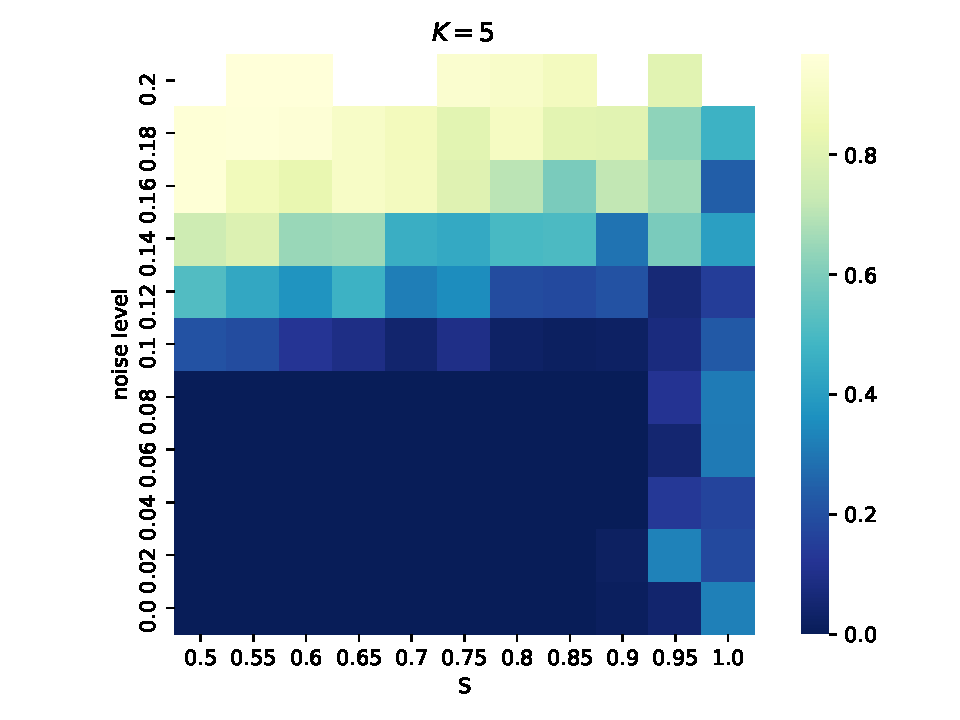
\includegraphics[width=\textwidth]{Figures/p_v_noise_k=5.pdf}
          \caption{}
      \end{subfigure} \\
  \caption{Final average polarization varies with both the width of the
    uniform distribution of initial opinion magnitudes and the noise level in
    the opinion updates. Noisy opinion updates can perturb the system away from
    situations where homogeneity of opinion would otherwise obtain. $K=2,3,4,5$
    are shown. The value in each square of the heatmap is the average of
    fifty trials. Each trial ran over 10k timesteps.
  }
  \label{fig:heatmaps}
\end{figure}



\section{Reproduction of results from Flache and Macy 2011}
\label{sec:label}

We are trying to recreate the first three figures from Experiment 2 of 
\citeA{Flache2011}, for the cases where negative valence was allowed.
See Section 3.2 starting on p. 166 in \citeA{Flache2011} for details of the
network structure, the two methods of network randomization used, and 
the structure of the experiments. See Section 2.1, starting on p. 151, for 
the introduction of the dynamical equations and outcome measures. Section 2.1
also contains asynchronous update rules (p. 155-156). Importantly, agent opinions
and weights are not updated on the same time step; only one or the other is
updated. Which one is updated is chosen at random. That and more fun details
are in the paper.

\begin{figure}
\begin{center}
  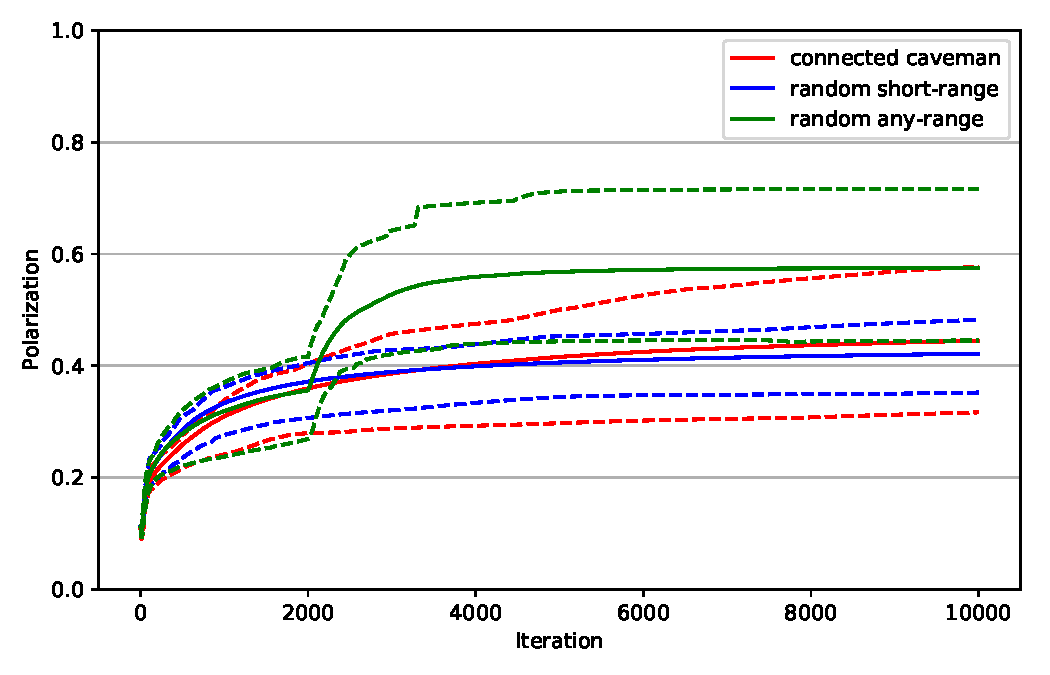
\includegraphics[width=\textwidth]{Figures/figure10b.pdf}
\end{center}
  \caption{Average of 50 trials with 25$^{\mathrm{th}}$ and 75$^{\mathrm{th}}$ 
    percentile values shown at each timestep (dashed line). Compare with
    Figure 10 of Flache and Macy (2011), p. 168.}
\label{fig:figure10-reproduction}
\end{figure}

\begin{figure}
\begin{center}
  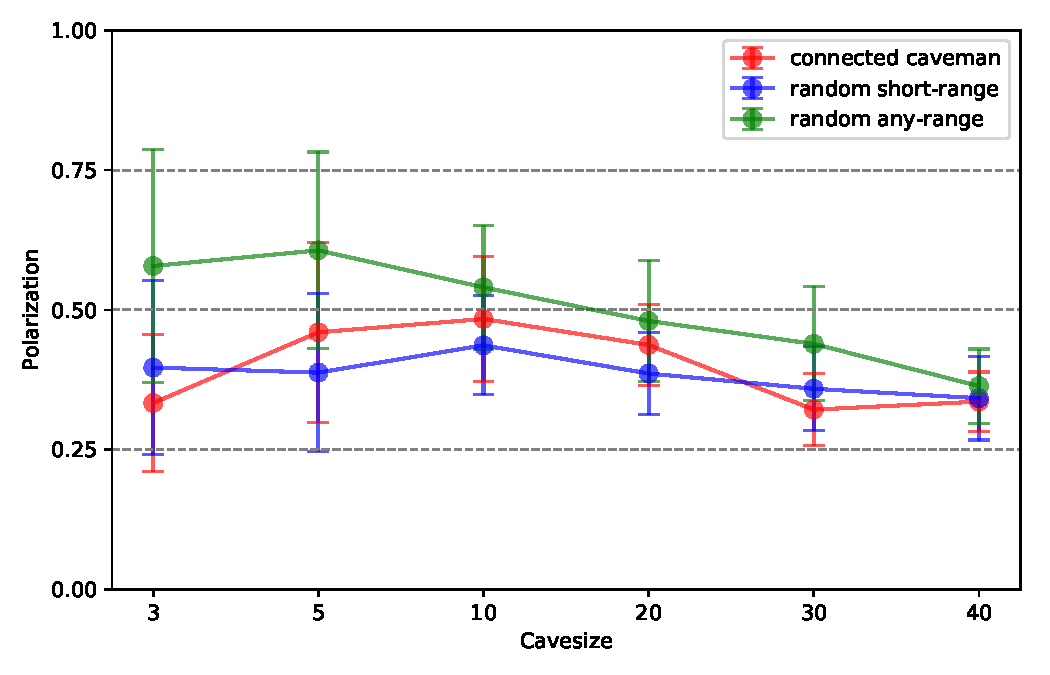
\includegraphics[width=\textwidth]{Figures/figure11b.pdf}
\end{center}
  \caption{The average of the polarization over 50 trials for varying cave size.
    Compare with Figure 11 of Flache and Macy (2011), p. 170.}
\label{fig:figure11-reproduction}
\end{figure}

\begin{figure}
\begin{center}
  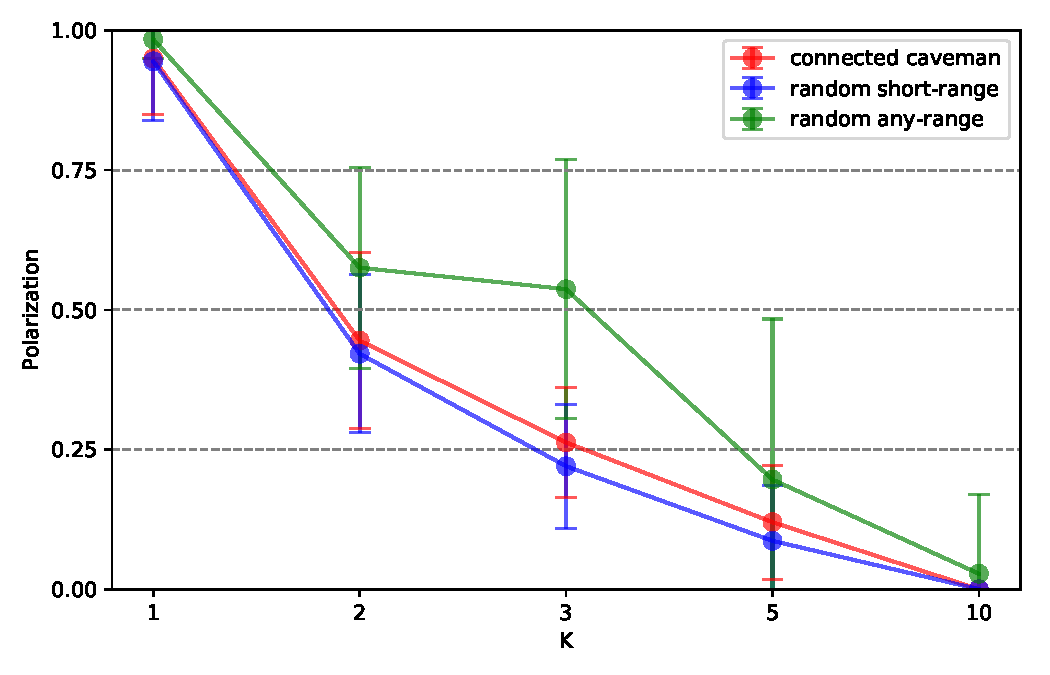
\includegraphics[width=\textwidth]{Figures/figure12b.pdf}
\end{center}
  \caption{Average polarization over 50 trials for different 
    ``cultural complexities,'' $K$. Compare to Figure 12 of Flache and Macy
    (2011), p. 171.}
\label{fig:figure12-reproduction}
\end{figure}



\bibliographystyle{apacite}

\setlength{\bibleftmargin}{.125in}
\setlength{\bibindent}{-\bibleftmargin}

\bibliography{/Users/mt/workspace/papers/library.bib}

\end{document}
